\documentclass{tietreport}

% Import images
\usepackage{graphicx}
\usepackage{amsmath}

% Bibliography configuration
\usepackage[
  date=year,
  style=alphabetic,
  backend=biber,
  sorting=nty,
  maxnames=5,
  minnames=3,
  maxalphanames=4,
  minalphanames=3,
  backref=true,
  doi=false,
  isbn=false,
  url=false,
  eprint=false
]{biblatex}
\addbibresource{references.bib}

%% ==================================================
%% PROJECT FIELDS
%% ==================================================

% Course/Lab header
\TitlePageHeader{%
  UCS503P - Software Engineering Project%
}

% Main project title
\ProjectTitle{%
  MATES%
}

% Subtitle or project description
\ProjectSubTitle{%
  A Taste Based Social Discovery Platform%
}

% Student information (up to 4 students)
\author{%
  Tulika Jain \quad \texttt{1024160110} \\
  Mukul \quad \texttt{1024160124} \\
  Pranav Tiwari \quad \texttt{1024160127}%
}

% Group number, degree, year, program
\TitlePageSubText{%
  BE Third Year, CSE%
}

% Faculty advisor/guide name
\AdvisorName{%
  Anushka Ma'am%
}

% Evaluation period and department info
\TitlePageFooterText{{%
    \large Mid-Semester Evaluation \\[0.2cm]
    \bfseries Computer Science and Engineering
    Department%
  } \\[0.15cm]
  Thapar Institute of Engineering and Technology,
  Patiala%
}

%% ==================================================

\begin{document}

% Generate title page
\maketitle

% Table of contents (auto-generated from chapters)
\tableofcontents

% ===== CHAPTER 1: INTRODUCTION =====

\chapter{Introduction}

\section{Background and Context}

Existing social platforms are typically organized around
a single content category such as music, photos, or short
video, or around a follower based model that optimizes for
reach rather than genuine compatibility. A person's taste
is usually spread across several disconnected apps, one for
music, one for movies, one for books, with no unified
representation of who they actually are. MATES addresses
this by translating cross domain taste similarity into a
measurable, explainable compatibility score, delivered
through a working mobile application.

\subsection{Problem Statement}

Users who want to find people who genuinely share their
taste face four recurring pain points:

\begin{itemize}[leftmargin=0.7cm]
  \item \textbf{Fragmentation:} taste signals for music,
    film, and books live in separate, disconnected apps.
  \item \textbf{Opaque recommendations:} existing
    ``suggested for you'' features rarely explain
    \emph{why} two users were matched, which erodes trust.
  \item \textbf{Follower centric design:} one directional
    following does not guarantee any shared interest,
    producing noisy, low relevance feeds.
  \item \textbf{Weak niche discovery:} users with specific
    or unusual combinations of interests struggle to find
    others who share that exact combination.
\end{itemize}

\section{Project Objectives}

\begin{enumerate}
  \item \textbf{Objective 1:} Deliver a working, end to end
    core loop: sign up, import taste, view ranked matches,
    see why the match was made, connect, and chat, all
    against live data.
  \item \textbf{Objective 2:} Make every compatibility
    score explainable by surfacing the specific shared
    items and divergence highlights behind it, rather than
    an opaque ranking.
  \item \textbf{Objective 3:} Extend the core loop with
    social features (content sharing, communities, and
    real time chat) so the app supports ongoing engagement
    rather than a single match event.
\end{enumerate}

% ===== CHAPTER 2: SYSTEM ARCHITECTURE =====

\chapter{System Architecture}

\section{High Level Design}

The system follows a mobile client talking to a REST
backend, which in turn talks to external taste data
providers and to the Claude API for narrative generation.
The core workflow is: a user authenticates, imports taste
keywords across music, movies, and books, and the backend
resolves each item against a live external provider. The
Compatibility Engine then scores the user against a
candidate pool using a weighted blend of similarity
measures, and returns a ranked, explainable Discovery
feed. A connection request that gets accepted unlocks chat,
and an AI generated conversation starter is offered
alongside it. Users can also post Content Drops from their
own taste, react to other people's drops, and join
tag based Communities suggested from their taste vector.
Figures \ref{fig:usecase} to \ref{fig:dfd2} document this
behaviour at increasing levels of detail.

\clearpage
\begin{figure}[p]
  \centering
  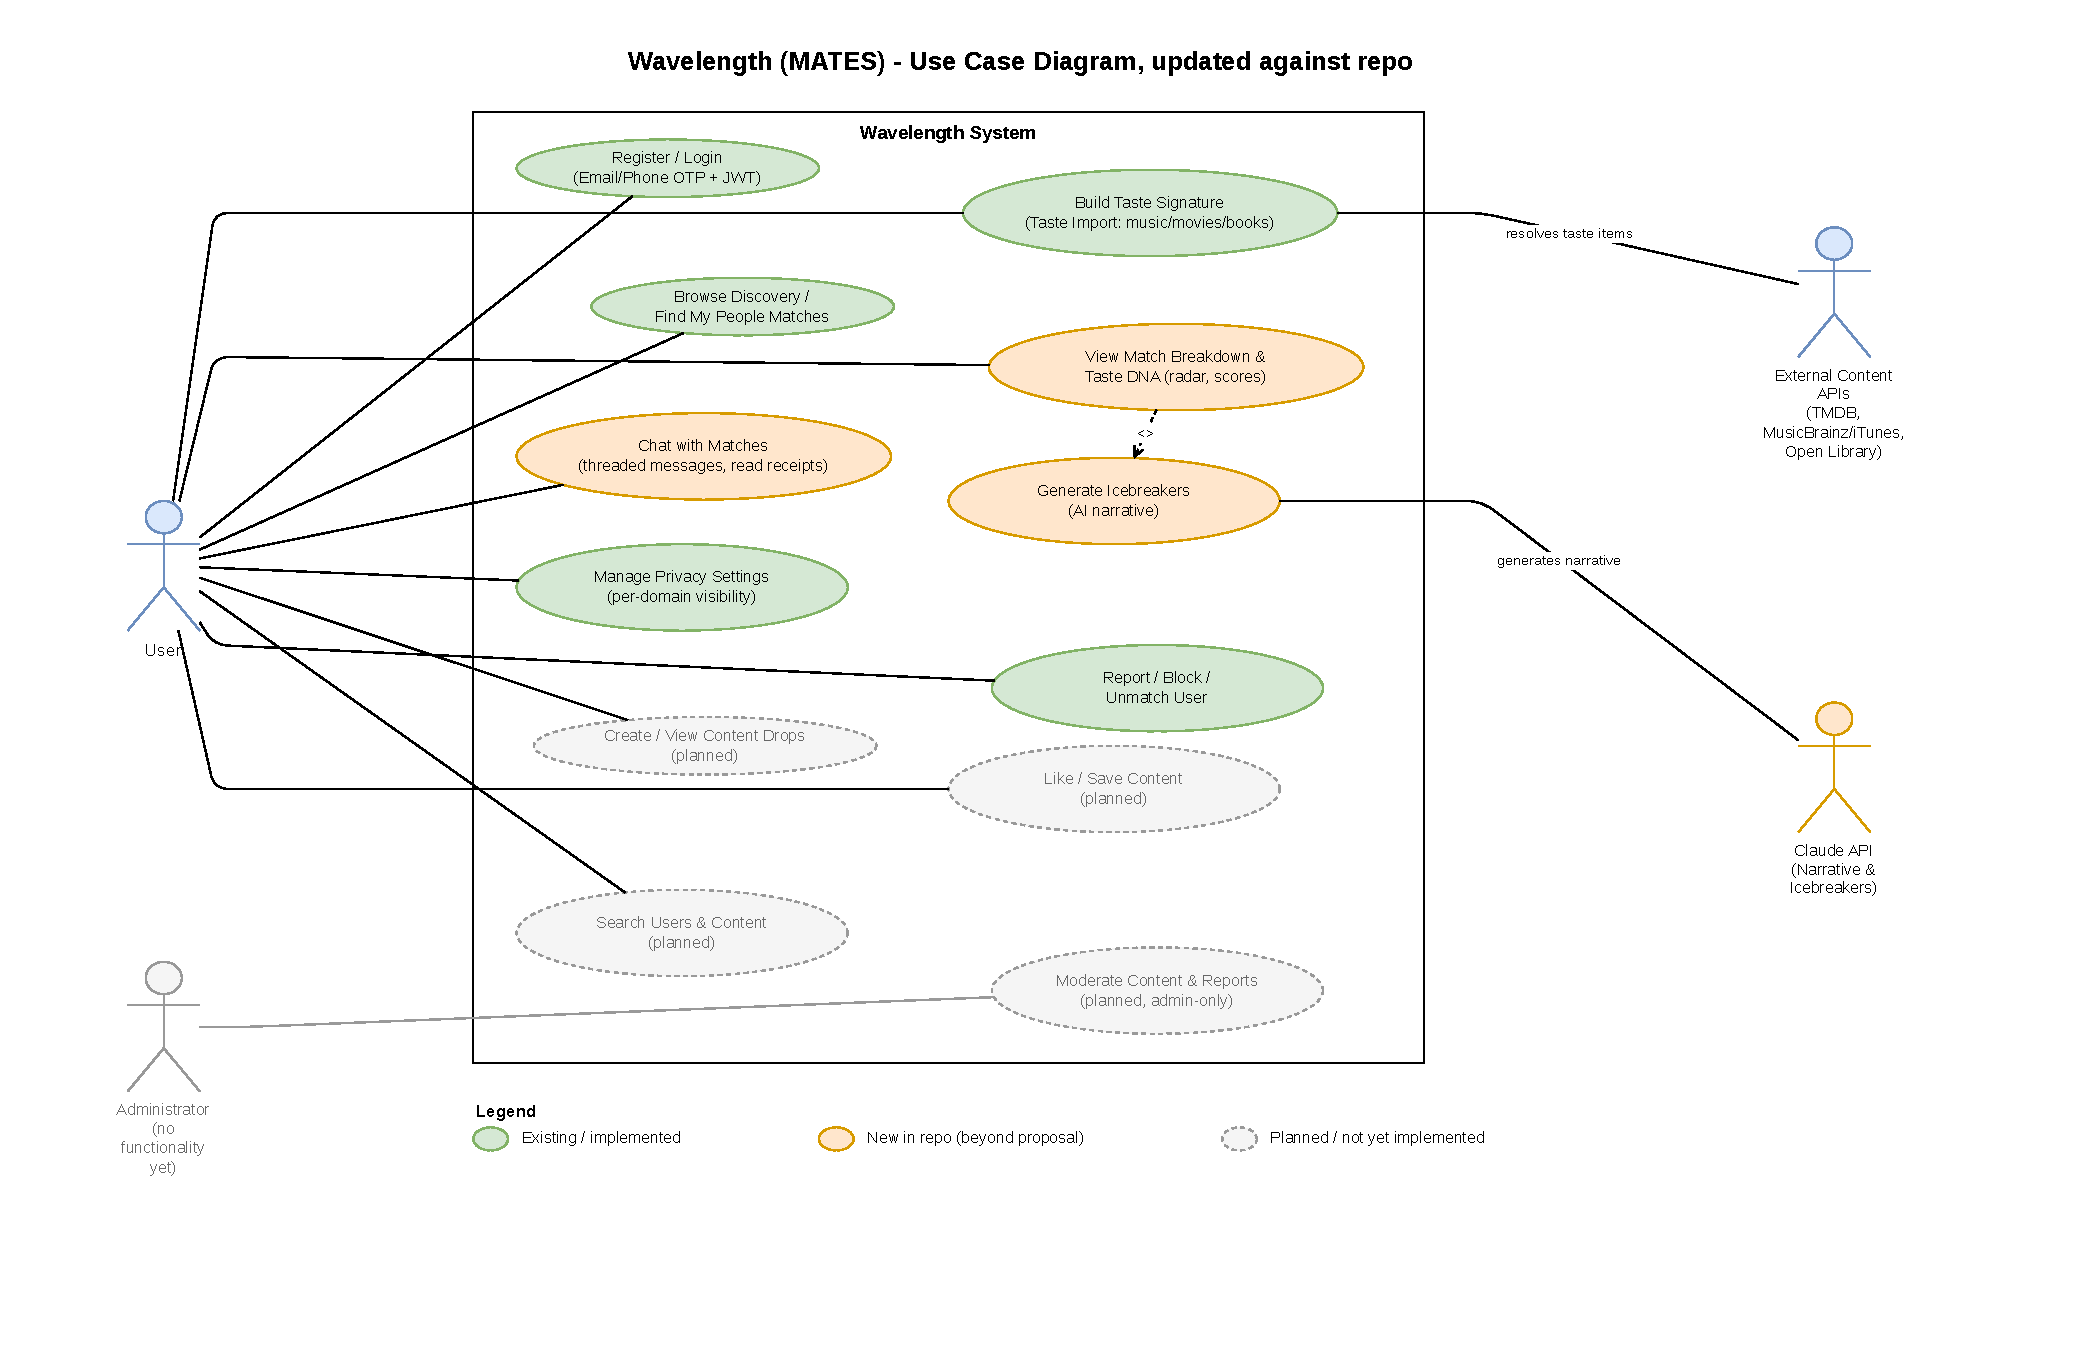
\includegraphics[width=0.95\textwidth]{figures/UseCaseDiagram_Updated_drawio.pdf}
  \caption{Use case diagram of the MATES system.}
  \label{fig:usecase}
\end{figure}
\clearpage

\clearpage
\begin{figure}[p]
  \centering
  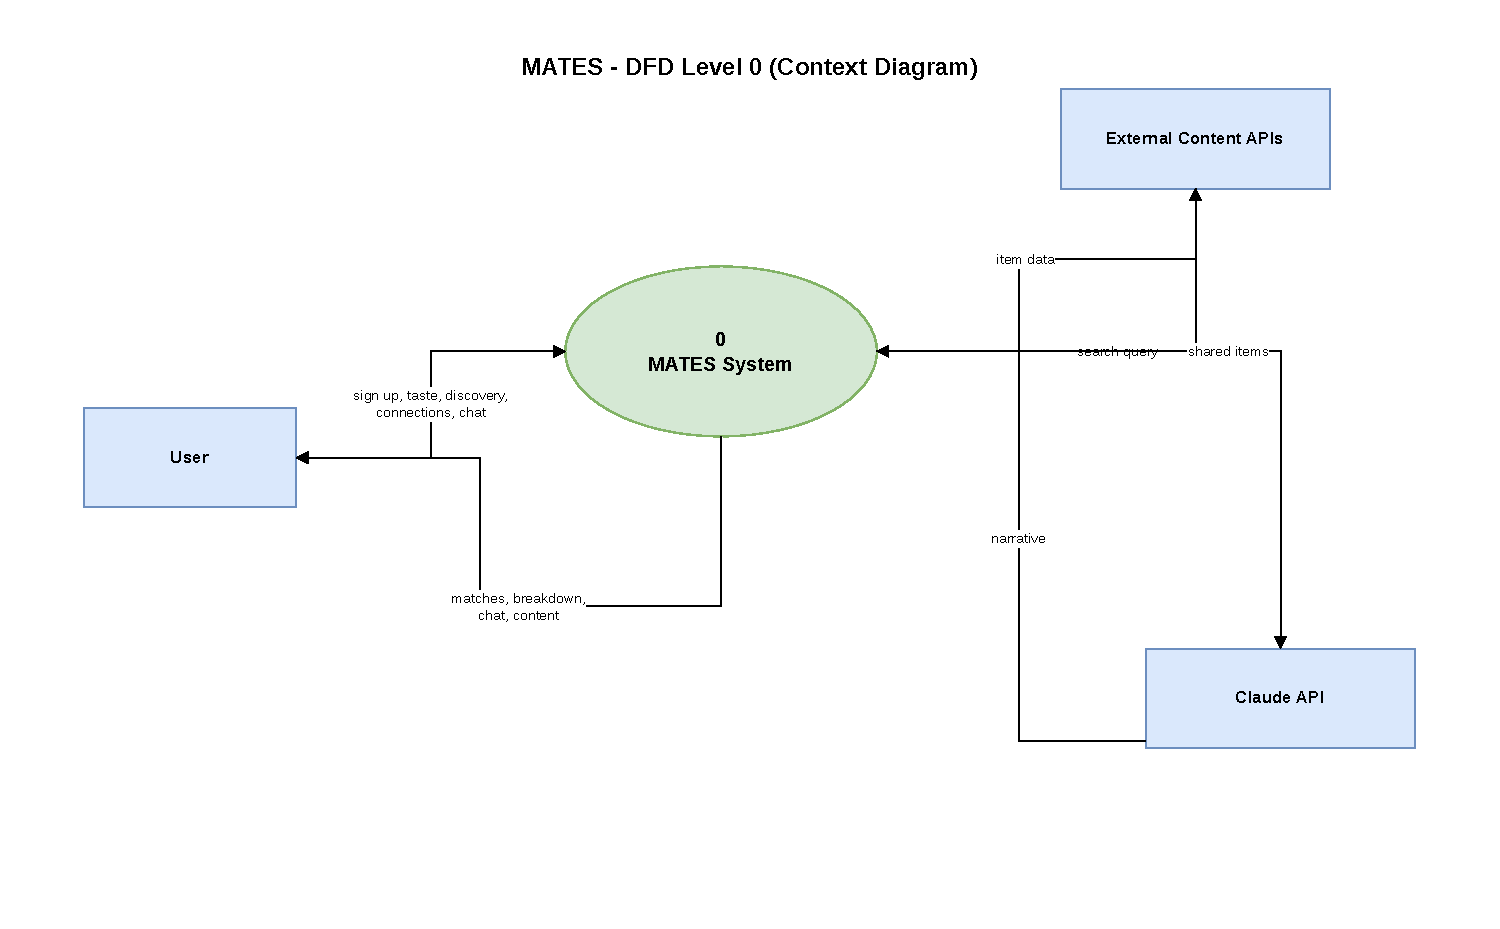
\includegraphics[width=0.9\textwidth]{figures/MATES_DFD_Level0_Clean_drawio.pdf}
  \caption{Data flow diagram, Level 0, context diagram.}
  \label{fig:dfd0}
\end{figure}
\clearpage

\clearpage
\begin{figure}[p]
  \centering
  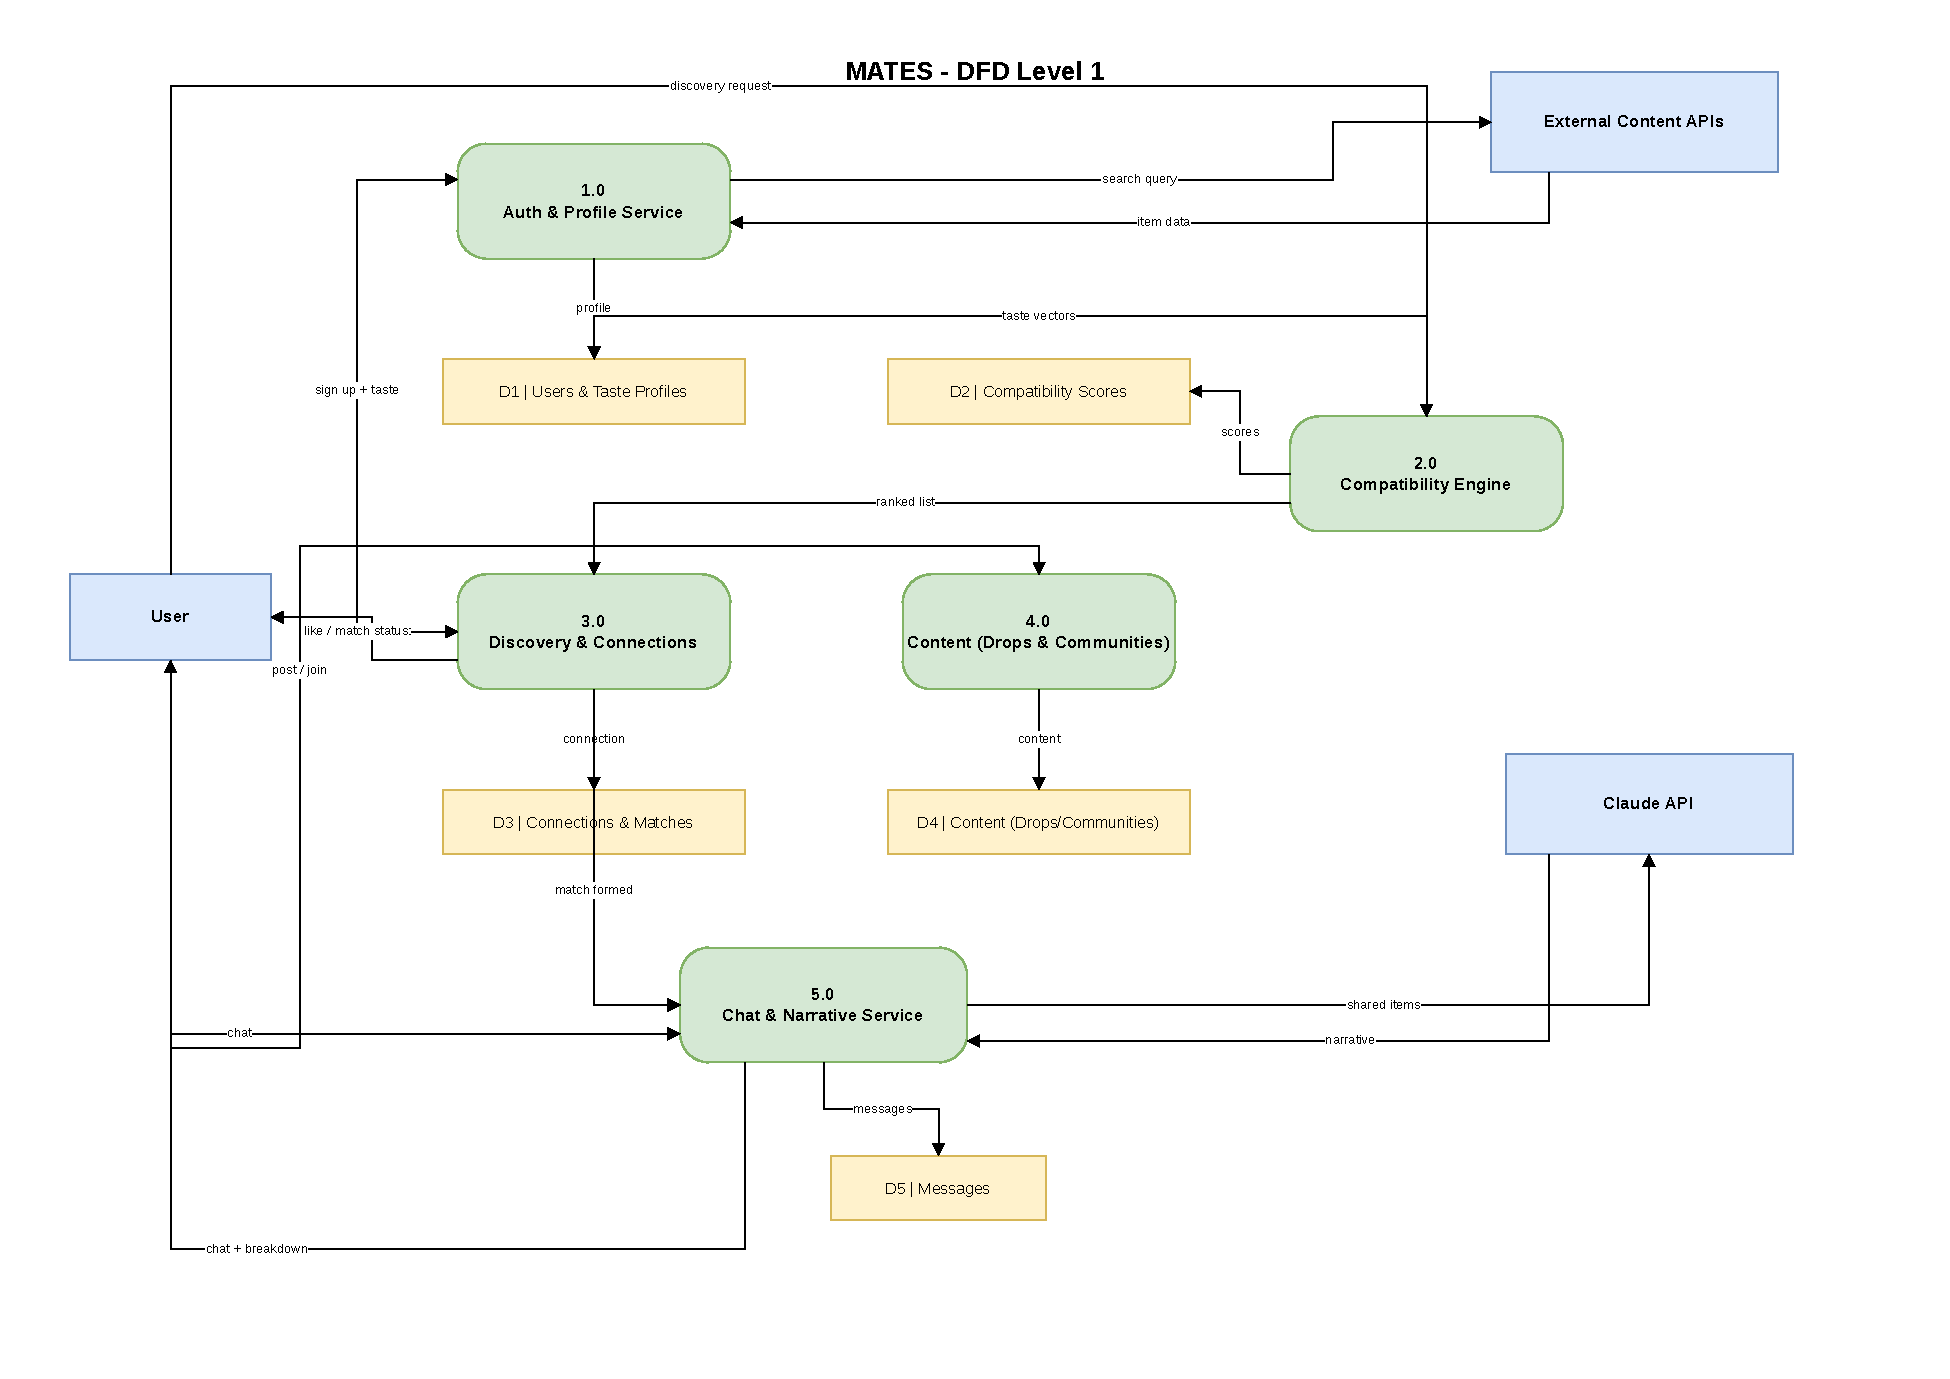
\includegraphics[width=0.95\textwidth]{figures/MATES_DFD_Level1_Clean_drawio.pdf}
  \caption{Data flow diagram, Level 1, showing the backend
    processes and data stores that make up the system.}
  \label{fig:dfd1}
\end{figure}
\clearpage

\clearpage
\begin{figure}[p]
  \centering
  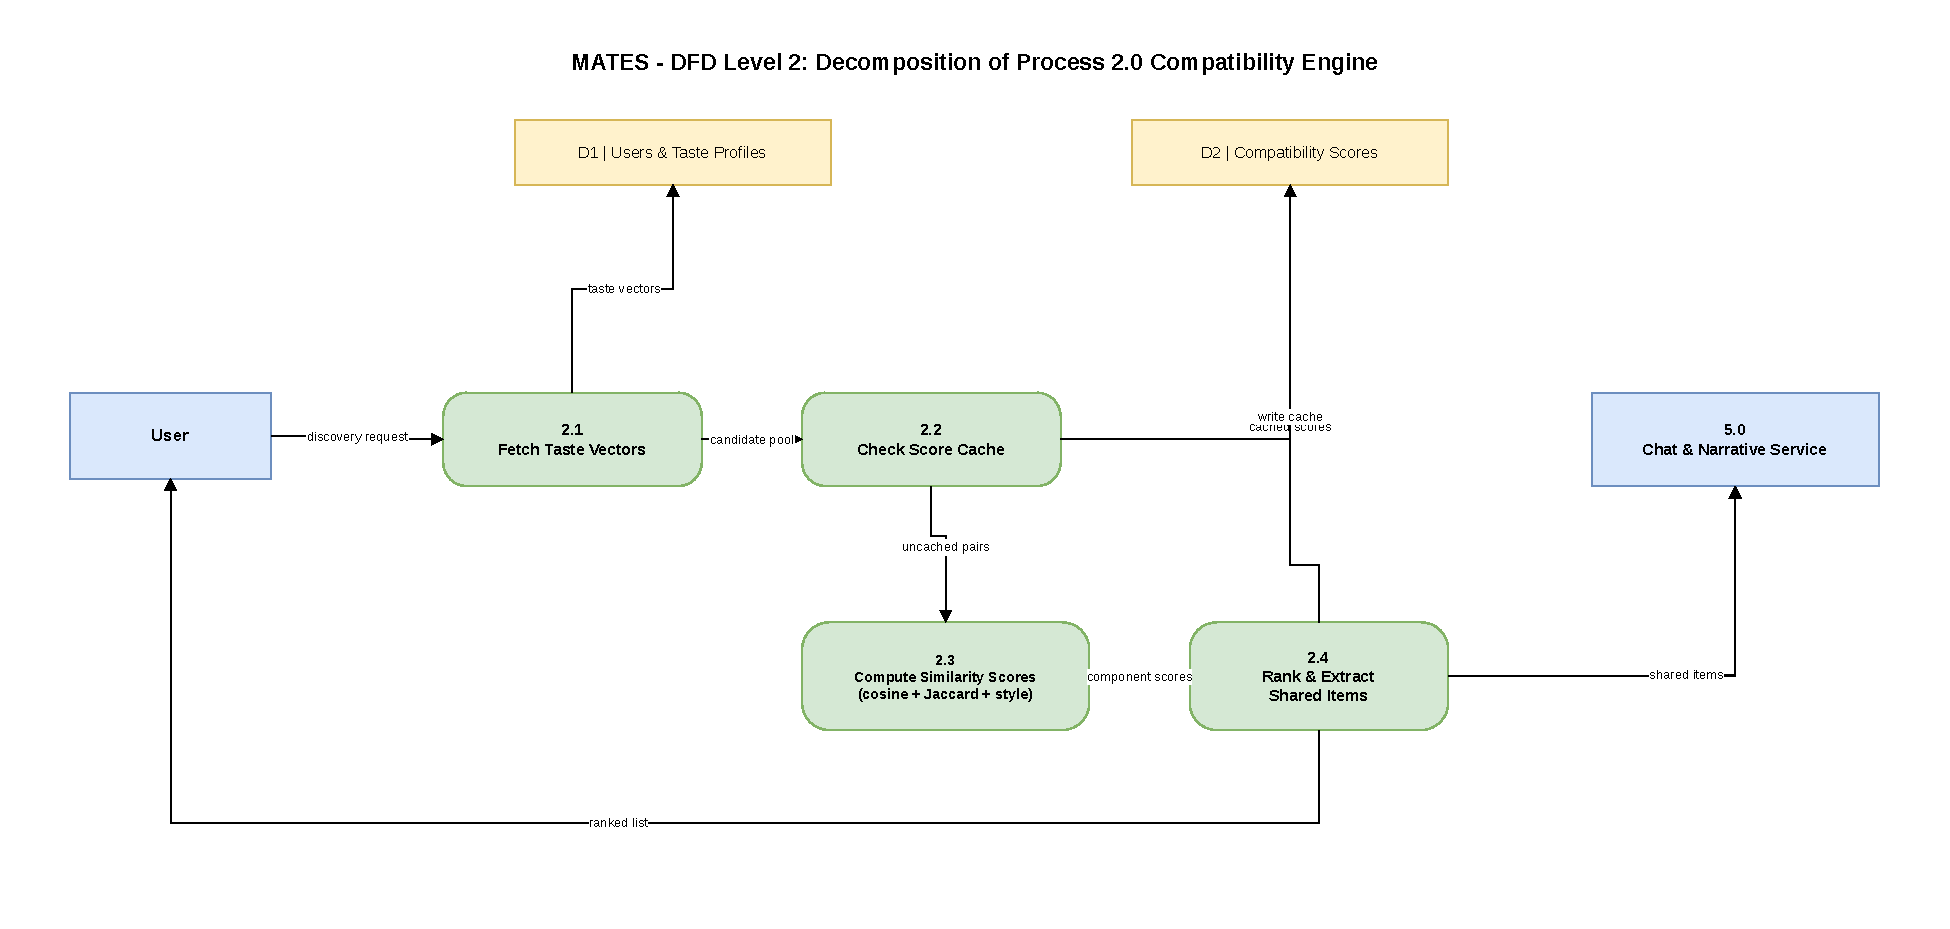
\includegraphics[width=0.85\textwidth]{figures/MATES_DFD_Level2_Clean_drawio.pdf}
  \caption{Data flow diagram, Level 2, decomposition of the
    Compatibility Engine process.}
  \label{fig:dfd2}
\end{figure}
\clearpage

\section{Implementation Details}

\subsection{The Compatibility Engine}

The compatibility engine lives in its own dependency free
module, with no database, HTTP, or framework code, so the
scoring algorithm can be developed and unit tested in
isolation. It computes, for a pair of users:
\[
  \text{score} = 0.45\times\text{cosine} +
                 0.35\times\text{weighted Jaccard} +
                 0.20\times\text{style alignment}
\]
where cosine similarity captures overall taste shape,
weighted Jaccard captures literal shared favourites, with
each shared item weighted by inverse popularity so two
people who both love an obscure film score far higher than
two who both love a blockbuster, and style alignment
captures era and mood overlap. Domain weights across
music, movies, and books are not fixed at a third each: a
domain counts only when both users have data in it, scaled
by data depth and each user's stated priority, so an
unconnected domain cannot silently drag a score toward
zero. Every score returned by the engine carries the
concrete shared items that produced it, plus divergence
highlights, the distinctive things one person loves that
the other has never touched, which double as conversation
prompts for the icebreaker feature.

\subsection{Feature Modules}

\begin{itemize}
  \item \textbf{Auth:} email and phone OTP, JWT issuance,
    and replay and brute force protection.
  \item \textbf{Onboarding:} name, age, city, bio, and
    stated intent (dating, friends, or both).
  \item \textbf{Taste import:} live search and add across
    all three launch domains.
  \item \textbf{Discovery:} a draggable, compatibility
    ranked card stack that is aware of the user's stated
    intent, with filters for minimum match and age.
  \item \textbf{Connections:} an opt in, bidirectional
    request and accept flow. A like sends a connection
    request; chat unlocks only once the other person
    accepts, and a mutual like accepts instantly.
  \item \textbf{Breakdown:} a score ring, per domain
    scores, the Taste DNA radar (five axes derived from
    the data, never self reported), an AI written
    narrative, and a share/differ toggle.
  \item \textbf{Narrative and icebreakers:} generated via
    the Claude API when an API key is configured, with a
    written in code fallback that still names real,
    concrete shared titles~\cite{anthropic-api}.
  \item \textbf{Content Drops:} short posts built from a
    user's own taste items, with like and save reactions,
    an optional community tag, and a ``you have this too''
    flag when a drop matches the viewer's own profile.
  \item \textbf{Communities:} tag based rooms with join and
    leave, suggestions ranked by the user's own taste tags,
    a member list, and a per community drop feed.
  \item \textbf{Chat:} threaded messages, read receipts,
    and taste based icebreakers, including seeded demo
    profiles that reply instantly for testing.
  \item \textbf{Add a profile:} a tool to build synthetic
    people by hand so they join the matching pool at once,
    used to seed a demoable Discovery feed.
  \item \textbf{Appearance:} dark, light, and system theme,
    persisted across sessions.
  \item \textbf{Safety:} block, report, and unmatch.
  \item \textbf{Privacy:} per domain visibility, set to
    full, aggregate, or hidden.
\end{itemize}

% ===== CHAPTER 3: UI/UX DESIGN =====

\chapter{UI/UX Design}

\section{Design Concept}

MATES is about the texture of what someone loves, so the
interface stays dark and low chroma and lets artwork and
type carry the colour. Three accent hues are reserved for
the three taste domains, music, movies, and books, and are
never used decoratively for anything else, so a colour
always means the same thing wherever it appears in the
app. A light theme mirrors the same geometry and type
scale, with the domain accents darkened slightly so they
stay legible on a pale background; the user can switch
between dark, light, and system at any time from Settings.

\begin{table}[h]
\centering
\begin{tabular}{|l|l|l|}
  \hline
  \textbf{Name} & \textbf{Hex} & \textbf{Usage} \\
  \hline
  Ink & \texttt{\#0E0D12} & App background, warm near black \\
  \hline
  Surface & \texttt{\#17161D} & Cards and input fields \\
  \hline
  Surface High & \texttt{\#232129} & Elevated surfaces, disabled states \\
  \hline
  Stroke & \texttt{\#2E2B36} & Borders and dividers \\
  \hline
  Cream & \texttt{\#F6F3EC} & Primary text \\
  \hline
  Muted & \texttt{\#8E8A9C} & Secondary text \\
  \hline
  Faint & \texttt{\#5E5A6B} & Tertiary text, low emphasis icons \\
  \hline
  Music accent & \texttt{\#6FE3C4} & Music domain, primary actions, ``like'' \\
  \hline
  Movie accent & \texttt{\#F2A65A} & Movie domain \\
  \hline
  Book accent & \texttt{\#B08CF0} & Book domain \\
  \hline
  Danger & \texttt{\#E5687A} & Destructive actions, ``pass'' or report \\
  \hline
\end{tabular}
\caption{Dark theme colour palette}
\label{tab:palette}
\end{table}

\section{Typography}

The base Material 3 type scale is overridden with a
tighter, more compact scale, tuned for a card heavy, data
dense interface. Display and headline styles use negative
letter spacing so large numerals and titles feel tight
rather than airy, and body styles use a slightly taller
line height for comfortable reading in chat and captions.

\begin{table}[h]
\centering
\begin{tabular}{|l|l|l|}
  \hline
  \textbf{Style} & \textbf{Size} & \textbf{Weight} \\
  \hline
  Display Small & 36 & 700 \\
  \hline
  Headline Medium & 27 & 700 \\
  \hline
  Title Large & 20 & 600 \\
  \hline
  Title Medium & 17 & 600 \\
  \hline
  Title Small & 15.5 & 600 \\
  \hline
  Body Medium & 15 & 400 \\
  \hline
  Body Small & 13.5 & 400 \\
  \hline
  Label Small & 11.5 & 600 \\
  \hline
  Match score numerals & 46 & 700 \\
  \hline
\end{tabular}
\caption{Type scale. Match score numerals additionally use
  tabular figures so the digits do not jitter as a score
  animates.}
\label{tab:type}
\end{table}

\section{Core Components}

\begin{itemize}
  \item \textbf{Score Badge:} renders a compatibility score
    with a colour that shifts along the palette as the
    score rises, from a faint grey at low compatibility to
    the music accent teal at a strong match.
  \item \textbf{Taste DNA Radar:} a five axis radar chart,
    built with \texttt{fl\_chart}, visualising a user's
    taste profile.
  \item \textbf{Tab Shell:} the five tab bottom navigation
    shared across Discover, Drops, Rooms, Matches, and
    Taste.
  \item \textbf{Entrance:} a staggered fade and slide in
    animation applied to list items as they load, used
    across Discovery, Drops, and Communities.
  \item \textbf{Page Shell:} a consistent page padding and
    scroll wrapper used by every tab.
  \item \textbf{Mates Mark:} the animated app mark shown on
    the splash screen while the session is restored.
\end{itemize}

\section{Feature to Screen Mapping}

\begin{table}[h]
\centering
\small
\begin{tabular}{|p{2.6cm}|p{5.4cm}|p{5.4cm}|}
  \hline
  \textbf{Screen} & \textbf{What It Does} & \textbf{Concept Exercised} \\
  \hline
  Sign In / Verify & Email/phone OTP request and verification & Authentication: OTP issuance, JWT, brute force protection \\
  \hline
  Onboarding & Collects name, age, city, bio, and intent & Input validation and user profile modeling \\
  \hline
  Taste / Taste Search & Live search and add across music, movies, books & External API integration (TMDB, MusicBrainz/iTunes, Open Library) \\
  \hline
  Discover & Compatibility ranked, swipeable card stack with filters & Consuming a recommendation and matching algorithm \\
  \hline
  Compatibility Breakdown & Score ring, per domain scores, Taste DNA radar, narrative & Data visualisation and AI generated content \\
  \hline
  Drops & Compose and share taste items, like/save, tag a community & Content feed and social interaction state \\
  \hline
  Rooms (Communities) & Join/leave, suggestions, member list, per room feed & Ranking by tag overlap \\
  \hline
  Matches & Pending requests and active conversations & Connection state machine: request, accept, chat unlock \\
  \hline
  Chat & Threaded messages, read receipts, AI icebreakers & Messaging model and AI integration \\
  \hline
  Settings & Appearance and per domain privacy & User preference persistence \\
  \hline
  Requests & Inbox of pending connection requests & Connection request and accept workflow \\
  \hline
  Add a Profile & Builds a synthetic profile for the matching pool & Data seeding for cold start mitigation \\
  \hline
\end{tabular}
\caption{Mapping of each screen to what it does and the
  concept it exercises}
\label{tab:screenmap}
\end{table}

% ===== CHAPTER 4: TECHNOLOGY STACK =====

\chapter{Technology Stack}

\begin{table}[h]
\centering
\begin{tabular}{|l|p{5.2cm}|p{5.2cm}|}
  \hline
  \textbf{Layer} & \textbf{Choice} & \textbf{Notes} \\
  \hline
  Mobile app & Flutter 3.47 / Dart 3.13~\cite{flutter} & Riverpod for state, go\_router for routing, dio for HTTP \\
  \hline
  Data visualisation & \texttt{fl\_chart} & Powers the Taste DNA radar chart \\
  \hline
  Backend API & Node.js 20+, TypeScript, Fastify 5~\cite{fastify} & REST endpoints, TypeBox schemas, generated OpenAPI contract \\
  \hline
  Database & PostgreSQL~\cite{postgresql} & PGlite (embedded WASM Postgres) for local development~\cite{pglite}, real Postgres in production \\
  \hline
  Auth & Email/phone OTP + JWT & Self implemented, no third party auth dependency \\
  \hline
  AI narrative & Claude API~\cite{anthropic-api} & Generates match narratives and icebreakers, with a code based fallback \\
  \hline
  Taste providers & MusicBrainz/iTunes, TMDB/Wikidata~\cite{tmdb}, Open Library~\cite{openlibrary} & Every domain resolves with zero required API keys \\
  \hline
  Testing & vitest (server), flutter\_test (app) & Server suite covers auth, compatibility, connections, drops, and communities \\
  \hline
  Contract & Generated OpenAPI document & Shared source of truth between the app and the server \\
  \hline
\end{tabular}
\caption{Technology stack}
\label{tab:stack}
\end{table}

\begin{table}[h]
\centering
\begin{tabular}{|l|l|l|}
  \hline
  \textbf{Domain} & \textbf{Primary provider} & \textbf{Fallback} \\
  \hline
  Music & MusicBrainz & iTunes \\
  \hline
  Movies & TMDB (if a key is configured) & Wikidata SPARQL \\
  \hline
  Books & Open Library & no fallback needed \\
  \hline
\end{tabular}
\caption{Taste data providers, all usable with zero required configuration}
\label{tab:providers}
\end{table}

% ===== CHAPTER 5: RESULTS & EVALUATION =====

\chapter{Results and Evaluation}

\section{Testing Methodology}

\begin{itemize}
  \item \textbf{Unit Testing:} the server test suite, built
    with \texttt{vitest}, covers authentication, the
    compatibility engine, connections, drops, and
    communities.
  \item \textbf{Integration Testing:}
    \texttt{api\_integration\_test.dart} exercises the real
    Dart client against a running server instance. It
    skips itself when the server is down, so
    \texttt{flutter test} stays green either way.
  \item \textbf{Static Analysis:} \texttt{flutter analyze}
    is run on the client with zero outstanding issues.
  \item \textbf{User Testing:} not yet run. A pilot with
    real users, supplemented by synthetic profiles to
    mitigate cold start, is planned for the next stage.
\end{itemize}

\section{Evaluation Metrics}

The following metrics are used to evaluate matching
quality once a pilot runs. Several are already
instrumented in the schema, since the underlying events are
timestamped as they happen.

\begin{table}[h]
\centering
\begin{tabular}{|p{5.2cm}|p{7.8cm}|}
  \hline
  \textbf{Metric} & \textbf{Status} \\
  \hline
  Match to connection rate & Instrumented: swipe and connection request events are timestamped \\
  \hline
  Connection acceptance rate & Instrumented: connection request status and response time are stored \\
  \hline
  Taste Signature completion rate & Instrumented: profile completeness is tracked per user \\
  \hline
  Match explanation density & Instrumented: shared highlights are stored per compatibility pair \\
  \hline
  Explainability satisfaction (1 to 5) & Needs an in app rating prompt, not yet built \\
  \hline
  Reliability / uptime & Needs a deployment target with monitoring, not yet built \\
  \hline
  Server unit tests & Passing, current suite covers auth, compatibility, connections, drops, communities \\
  \hline
  \texttt{flutter analyze} issues & Zero issues, as reported by the client build \\
  \hline
\end{tabular}
\caption{Evaluation metrics and current status}
\label{tab:metrics}
\end{table}

\section{Analysis}

\textbf{Did the team meet its objectives?} Objective 1 is
met: the core loop, sign up, import taste, see who matches,
see why, connect, and chat, works end to end against live
data. Objective 2 is met by construction, since the
compatibility engine cannot return a score without also
returning the shared items and divergence highlights behind
it. Objective 3 is met: Content Drops, Communities, and
Chat are all built and reachable from the main tab shell,
extending the app beyond a single match event into ongoing
engagement.

\textbf{Design decisions and how they were resolved.} The
backend uses Fastify with TypeScript so the API and the
generated contract share one language end to end.
PostgreSQL was chosen because the data is fundamentally
relational, pairs, requests, and memberships, and database
constraints catch real bugs such as an ordered pair
violation or a self swipe. Authentication is a self hosted
OTP and JWT flow, which keeps the whole project runnable
without any third party accounts or keys. Profile portraits
are currently generated rather than uploaded, so the app
has a complete, demoable visual identity for every user
without needing an upload pipeline yet. On the toolchain
side, iOS and Android builds are currently blocked by an
incomplete Xcode installation and a missing Android SDK on
the development machine, so a web target was added to the
Flutter project purely to verify the UI in the meantime.

% ===== CHAPTER 6: CONCLUSION =====

\chapter{Conclusion}

\section{Summary of Work}

MATES implements a cross domain Taste Signature feeding an
explainable compatibility score, delivered as a working
mobile application with a tested backend engine. The core
discovery to chat loop is complete and running against live
external data sources, and the social layer around it,
Content Drops, Communities, and Chat, is built and
reachable from the main navigation.

\section{Key Findings}

\begin{itemize}
  \item \textbf{Finding 1:} An explainable compatibility
    engine, cosine similarity, inverse popularity weighted
    Jaccard overlap, and style alignment combined at fixed
    weights, is straightforward to keep dependency free and
    unit testable, which made it safe to build social
    features such as Chat and Drops on top of it with
    confidence.
  \item \textbf{Finding 2:} Choosing self hosted or key free
    equivalents for authentication and taste data providers
    kept the whole stack runnable with zero external
    accounts, which made local development and demoing
    straightforward.
  \item \textbf{Finding 3:} Instrumenting evaluation events,
    swipes, connection requests, and profile completeness,
    from the start means the metrics needed for a pilot are
    already collectible; what remains is running the pilot
    itself and building the rating and monitoring surfaces
    around it.
\end{itemize}

\section{Future Work and Recommendations}

\begin{enumerate}
  \item Continue building out the content part of the app,
    Taste Rooms, Blind Taste Mode, Collaborative Blends,
    and a Weekly Recap, for which schema support already
    exists.
  \item Implement in app Search across users and content,
    and an Admin/Moderation dashboard for reviewing reports
    and flagged content.
  \item Build the notification layer for connections,
    likes, and new matches.
  \item Add an in app explainability rating prompt so the
    1 to 5 clarity metric can be collected from real users.
  \item Move the compatibility score from a per request
    cache to a nightly precompute job once user volume
    justifies it.
  \item Add Spotify OAuth for listening history and audio
    features, to complete the music vector's sonic
    fingerprint.
  \item Implement a real photo upload pipeline; the schema
    and moderation columns already exist, and portraits are
    currently generated rather than uploaded.
  \item Replace console logged OTPs with a real SMS or
    email delivery provider.
  \item Complete iOS and Android toolchain setup so the app
    can move off the temporary web target and onto real
    devices.
  \item Stand up a CI/CD pipeline, automated build, backend
    tests, linting, and staging deployment, and a real
    deployment target so reliability and uptime can be
    measured.
  \item Run the planned pilot with real users, supplemented
    by synthetic profiles, and use it to validate the
    evaluation metrics end to end.
\end{enumerate}

\section{Final Remarks}

The project validates its core engineering bet, that a
lightweight, explainable, cross domain compatibility score
is enough to drive a working discovery to connection loop
without needing a research grade matching model, and that
the same foundation supports an active social layer on top
of it. The remaining work is concentrated in deeper content
features, search, moderation tooling, and deployment,
rather than in the matching core itself, which is a
reasonable place to be at the mid semester stage.

% ===== BIBLIOGRAPHY =====

% Print bibliography with heading in TOC
\printbibliography[heading=bibintoc]

\end{document}
